\documentclass[11pt, journal]{IEEEtran}
\usepackage{lipsum}
\usepackage[T1]{fontenc}
\usepackage{fouriernc}
\usepackage{cases}
\usepackage{amsmath}
\usepackage[noadjust]{cite}
\usepackage{hyperref}
\usepackage{multirow}
\usepackage{graphicx}
\usepackage{adjustbox}
\usepackage{makecell}
\usepackage[dvipsnames]{xcolor}
\usepackage{tikz}
\usepackage{lipsum}
\usepackage{listings}

\hypersetup{
    colorlinks=true,
    linkcolor=blue,
    anchorcolor=blue,
    urlcolor=blue,
    citecolor=blue
}

\newcommand{\eq}{\; = \;}
%\newcommand{\text}[1]{\mbox{\footnotesize #1}}
\newcommand{\nl}{

\medskip

}
\newcommand{\centered}[2]{\begin{tabular}{#1} #2 \end{tabular}}

\lstdefinestyle{standstyle}{
    %backgroundcolor=\color{backcolour!05},
    basicstyle=\ttfamily\linespread{1}\scriptsize\color{black!80},
    breakatwhitespace=false,
    breaklines=true,
    captionpos=b,
    keepspaces=true,
    numbers=none,
    numbersep=5pt,
    showspaces=false,
    showstringspaces=false,
    showtabs=false,
    tabsize=4,
}

\lstset{style=standstyle}

\newcommand{\nl}{

\medskip

}

\DeclareMathAlphabet{\mathcal}{OMS}{zplm}{m}{n}

\title{\texttt{/gamerule doFireTick true}\\A binary classifier for recognizing fire}
\author{Leonardo Biason (\textit{2045751}) \quad Lorenzo Marinelli (\textit{2043092}) \quad Oscar Michele Norelli (\textit{2046721})}

\begin{document}

\maketitle

\begin{abstract}
    This article contains the report for the Deep Learning course challenge, which asked to the course participants to build a binary classifier which should recognize whether there is some fire in a picture. We here present a possible implementation of this classifier, which reached an astonishing accuracy of $\mathbf{98.78\%}$
\end{abstract}

\begin{keywords}
    Sapienza, AcsAi, CNN, ResNet, Deep Learning, Computer Vision 
\end{keywords}

\section{Introduction}

CNNs have been widely adopted in many uses as of today, either for accessibility features or as useful detection tools. Many examples of medical emplyments exist, and that's only one of the many possible use cases. However, this kind of technology can also be useful when detecting dangers and perils, and for automating checking routines. We may consider CNNs as a type of sensor, which reacts to certain visual events. With this paper, we present a possible use case for CNNs, in particular, one tied to fire prevention.
\nl
\indent Fire prevention is usually ensured thanks to smoke sensors, which cover small areas and allow for a granular control of reduced ambients. However, this is only possible when the ambient is a closed one, and it's hard to apply this kind of techniques on open spaces. That is where CNNs may well fit: by using a visual sensor on open areas, it becomes easier to control larger areas for fire hazards, and to alert any competent autority when a fire breaks.
\nl
\indent This is ultimately the scope of this paper: to present a working model which can be employed for simple fire detection tasks. We will here explain the structure used, and the performance reached by the model.
\nl
In order to perform the given task, we decided to use an ensemble of three models, and to train them with a dataset which has been previously augmented by manipulating all the images.

\section{Structure of the dataset}

\begin{figure}
    \label{dataset_example}
    \centering
    \begin{tabular}{c c}
        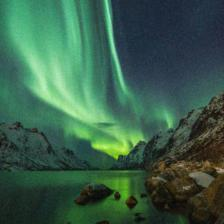
\includegraphics[width = 3.5cm]{imgs/no_fire.jpg} & 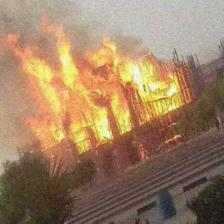
\includegraphics[width = 3.5cm]{imgs/fire.jpg}
        \\
        \texttt{label: 0} & \texttt{label: 1}
    \end{tabular}
    \caption{Example of images belonging to the dataset with the corresponding label}
\end{figure}

For this task, we used a dataset composed of $10,926$ images; we later applied some steps of data augmentation so that we could achieve better results by making the model generalize enough.
\nl
The dataset is separated in two folders (for the two classes), where each folder represents the label of each image:
\begin{itemize}
    \item folder \verb|0| contains the images that do not contain fire;
    \item folder \verb|1| contains the images that contain fire;
\end{itemize}

\subsection{Data augmentation}

Data augmentation is a common step which is usually made to enhance the number of items in a dataset by using items already belonging to said dataset. We applied the following operations to our dataset:
\begin{itemize}
    \item \textbf{Random rotation}: to each image, a random rotation of $x$ degress could've been applied, where $x \in [0, 15]$. This ensures that the fire would be recognized even if it was not "parallel" with respect to the $y$ axis of the image;
    \item \textbf{Color jitter}: a random color jitter was also applied to all the images. The parameters passed to the jitter function are listed on Table \ref{color_jittering_vals}. By applying a color jitter, we make sure that the model would recognize a fire also when light conditions were not optimal in the photo (for instance if the image is either too dark or too bright);
    \item \textbf{Brightness noise}: for each image also some noise was added, and this was applied through a lambda function. For each image, some noise of equal size would be generated, and then through clamping the noise got applied to the image. This kind of noise allowed us to train the model to recognize a fire also in some harsh conditions, and helps avoiding overfitting.
\end{itemize}
\nl
After augmenting the whole dataset, the amount of samples went from $10,926$ to $21,852$, doubling the size of the dataset and allowing the models to train and reach more efficient results.

\begin{table}
    \caption{Parameters of the color jittering function}
    \label{color_jittering_vals}
    \centering
    \begin{tabular}{|l|c|}
        \hline
        \makecell{\textbf{Parameter}} & \textbf{Value}
        \\ \hline\hline
        \verb|brightness| & 0.2 \\ \hline
        \verb|contrast| & 0.2 \\ \hline
        \verb|saturation| & 0.2 \\ \hline
        \verb|hue| & 0.1 \\ \hline
    \end{tabular}
\end{table}

\section{Structure of the ensemble}

\begin{table*}
    \renewcommand{\arraystretch}{1.3}
    \caption{Structure of the ensemble}
    \label{ensemble_specs}
    \centering
    \begin{tabular}{|c|c|c|c|c|}
        \hline
        \makecell{\textbf{Model}} & \makecell{\textbf{Layer}} & \textbf{Dimensions} & \textbf{Loss} & \textbf{Optimizer} \\
        \hline
        \hline
        \multirow{4}{*}{ResNet 152} & \multicolumn{2}{c|}{Backbone of the ResNet 152} & \multirow{4}{*}{Focal Loss} & \multirow{4}{*}{AdamW}
        \\ \cline{2-3} 
        & Linear & $(1024 \times 512)$ & &
        \\
        & Linear & $(512 \times 2)$ & &
        \\
        & ReLU & / & &
        \\
        \hline \hline
        \multirow{1}{*}{ResNet 18} & \multicolumn{2}{c|}{Backbone of the ResNet 18} & \multirow{1}{*}{/} & \multirow{1}{*}{/}
        \\
        \hline\hline
        \multirow{1}{*}{ResNet 50} & \multicolumn{2}{c|}{Backbone of the ResNet 50} & \multirow{1}{*}{/} & \multirow{1}{*}{/}
        \\
        \hline
    \end{tabular}
\end{table*}

The ensemble is composed of three models, based on a ResNet 150, a ResNet 18 and a ResNet 50. The complete specifications of the three models can be found in Table \ref{ensemble_specs}. Some small modifications have been made to each model, in order to achieve different results. We here list all the modifications that have been made to each model, alongside an explanation of why they have been applied.

\subsection*{Model 1 \texorpdfstring{\textbullet}{•} ResNet 150}

% model ensemble: 
% - resnet152
% - resnet18
% - resnet50

\lipsum



\section{Performance evaluation}

\lipsum

\end{document}